\subsection{Unsupervised Techniques}
\label{unsupervised}

% ------------------------------------------------------------------------------

\subsubsection{Laplacian Eigenmaps (LEM)}
\label{laplace}

The reason for LEM to appear in this report alongside the LLE family is its 
underlying theory both providing a foundation for LLE \citep{belkinniyogi2003}, 
which was originally proposed lacking such, and closely relating to the 
theoretical concepts in HLLE \citep{donohogrimes2003}.

LEM are centered around the preservation of locality, i.e., mapping nearby
inputs to nearby outputs.
Locality is enforced via the \textit{Laplace-Beltrami operator} defined on
smooth, compact manifolds, and operationalized by means of the \textit{graph Laplacian} acting as a discrete approximator \citep{belkinniyogi2003}.
This idea is best understood recalling that the similarity of outputs for
similar inputs is essentially a notion of smoothness and can thus be controlled
by a size constraint on the gradient of the mapping function.
\\

\textbf{Laplace-Beltrami operator.}
Consider the twice differentiable function $f: \mani \rightarrow \R$ mapping
two points $\pv, \qv \in \mani$ to $f(\pv)$ and $f(\qv)$, respectively.
On $\mani$ these points are connected by a length-parametrized curve $c(t)$.
Denote the geodesic distance between $\pv$ and $\qv$ by $\ell$, such that
$\pv = c(0)$ and $\qv = c(\ell)$.

\begin{minipage}[b]{0.65\textwidth}
  Gradients of $f$ with respect to $\pv$ are defined in the local tangent space
  $T_{\pv}(\mani)$ spanned by vectors tangent to $\mani$ at $\pv$.
  As $\mani$ is embedded in $\RD$, its tangent spaces are Euclidean and of
  dimension $d$, i.e., $d$-dimensional hyperplanes \citep{sudderth2002} as
  depicted in figure \ref{fig:sphere-tangent}.
  If $\pv$ is identified with the origin of $T_{\pv}(\mani)$, the tangent space
  inherits an orthonormal coordinate system obtained from endowing
  $T_{\pv}(\mani)$ with the inner product from $\Rd$ \citep{donohogrimes2003}.
  With this, the distance $|f(\pv) - f(\qv)|$ of mappings can be expressed as
  the length of the integral
  $\int_0^{\ell} \langle \nabla f(c(t)), c^{\prime}(t) \rangle dt$.
  In other words, the geodesic curve connecting $\pv$ and $\qv$ is projected
  onto $T_{\pv}(\mani)$, and the length of this projection depends on the
  gradient of $f$ and the curve velocity.
\end{minipage}
\begin{minipage}[b]{0.05\textwidth}
  \phantom{xxx}
\end{minipage}
\begin{minipage}[b]{0.3\textwidth}
  \begin{figure}[H]
    \centering
    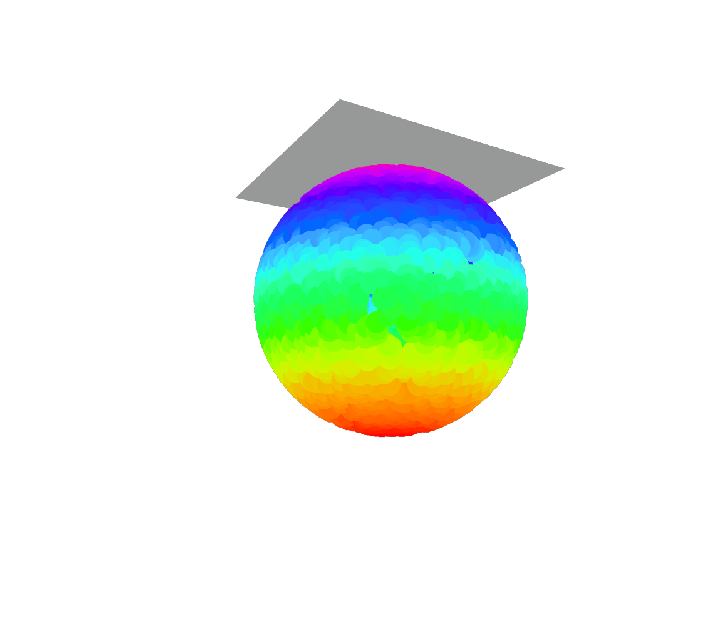
\includegraphics[trim = 90 70 60 30, clip, % left bottom right top
      width = 0.8\textwidth]{figures/sphere-tangent}
    \caption[Tangent hyperplane for two-dimensional unit sphere]{Tangent
    hyperplane for an exemplary point on the two-dimensional unit sphere
    manifold, embedded in $\R^3$. \textit{Source:} own representation.}
    \label{fig:sphere-tangent}
  \end{figure}
\end{minipage}

\vspace{0.5cm}

Exploiting the Schwartz equality and relations formally proved by
\citet{belkinniyogi2008}, it
can be shown that
$|f(\pv) - f(\qv)| \leq \| \nabla f(\pv) \| \cdot \| \pv - \qv\| + o$, where
$o$ marks a term of vanishing size.
As the distance between $\pv$ and $\qv$ is a datum,
$\| \nabla f \|$ controls how far apart points are mapped on the real line.
Consequently, the goal is to find a mapping that, on average, preserves
locality by posing a second-order penalty on $\| \nabla f \|$ and minimizing $\int_{\mani}\| \nabla f \|^2$.
This is just equal to minimizing $\int_{\mani} \mathcal{L}(f)f$ with the
Laplace-Beltrami operator $\mathcal{L}$ \citep{belkinniyogi2003}.
Applying the operator $\mathcal{L}$ to $f$ results in a function from the
same function space as $f$, and for $\mathcal{L} f = \lambda f$, $f$ is an
eigenfunction of $\mathcal{L}$ with $\lambda \in \R$ as its associated
eigenvalue.
Crucially, these eigenfunctions are orthogonal for $\mathcal{L}$ and their
eigenvalues are real, meaning they are natural candidates for forming a
functional basis \citep{levy2006}.
The optimal embedding map is then given by the $d$ principal eigenfunctions of
$\mathcal{L}$ after removing the bottom one which would map $\mani$ to a
single point \citep{belkinniyogi2003}.
\\

\textbf{Graph Laplacian.}
Now the same reasoning can be applied to the neighborhood graph approximation of
$\mani$.
Recall the desideratum of mapping nearby inputs to nearby 
outputs.
LEM achieves this by assigning edge weights\footnote{
These weights stem from the heat kernel intimately related to the 
Laplace-Beltrami operator and ensure positive semi-definiteness of the resulting
graph Laplacian. 
As an alternative, \citet{belkinniyogi2003} propose a simpler kernel that is 
equal to 1 for connected nodes and 0 otherwise.
}

\begin{equation*}
  w_{ij} = \begin{cases}
    \exp(\frac{\|\x_i - \x_j \|^2}{t}), t \in \R, & \mbox{ if } \x_i, \x_j
    \text{ are connected,} \\
    0 & \mbox{ otherwise,}
  \end{cases}
\end{equation*}

forming a weight matrix $\W = (w)_{ij} \in \R^{N \times N}$.
Clearly, edges between closer points receive larger weights.
A second matrix $\D = (d)_{ij} \in \R^{N \times N}$ takes the row
sums of $\W$ on its diagonals.
Penalizing output disparities more severely for pairs of nearby points, i.e.,
pairs with a large weight coefficient, the smoothness requirement may be stated
as follows:

\begin{equation*}
  \begin{split}
    \min_{\Y} \sum_{i, j} \| \y_i - \y_j \|^2 w_{ij}
    &= \min_{\Y} \sum_{i, j} \y_i^T \y_i w_{ij} + \y_j^T \y_j
    w_{ij} -
    2 \y_i^T \y_j w_{ij} \\
    &= \min_{\Y} \sum_i \y_i^T \y_i d_{ii} + \sum_j \y_j^T \y_j
    d_{jj} - 2 \sum_{i, j} \y_i^T \y_j w_{ij}.
  \end{split}
\end{equation*}

Now, define the graph Laplacian as
$\Lap = \D - \W \in \R^{N \times N}$, thereby coercing
all information about the graph structure into a single matrix
representation\footnote{
This corresponds to the general matrix $\M$ introduced in chapter
\ref{motivation}; the deviating notation shall merely emphasize the special
role of $\M$ as the Laplacian.}.
With $\Lap$ the above can be rewritten as

\begin{equation}
  \min_{\Y} \text{\textit{trace}}(\Y^T \Lap \Y), \quad \text{s.t. } 
  \Y^T \D \Y = \I,
  \label{eq-obj-lem}
\end{equation}

which has precisely the form of the generalized eigenvalue problem in equation
\ref{eq-gevproblem} and is therefore solved by eigendecomposition of $\Lap$ \citep{belkinniyogi2003}.
As in the continuous case, the bottom eigenvector with zero eigenvalue is
constant and must be discarded.
The subsequent $d$ eigenvectors yield the desired low-dimensional
embedding \citep{levy2006}.

% ------------------------------------------------------------------------------

\subsubsection{Locally Linear Embedding (LLE)}
\label{lle}

In proposing LEM, \citet{belkinniyogi2003} also demonstrated how the somewhat 
earlier LLE algorithm may be reinterpreted within the LEM framework: it can be 
shown to approximate the graph Laplacian under certain conditions and thus 
asymptotically approach the Laplace-Beltrami operator.
More recent research, however, suggests that these conditions might be more 
restrictive than previously assumed. 
In particular, convergence appears to depend on the choice of a regularization 
parameter required in the case of $D < k$ \citep{wuwu2018}.
\\

\textbf{Idea.}
The initial proposal by \citet{roweissaul2000}, ignorant to these findings, 
was made with a different, and rather heuristically motivated, intuition.
LLE relies on a simple yet powerful idea.
Each point $\x_i$ in the $D$-dimensional input space is expressed as a convex 
combination of its neighbors, such that the weighting coefficients of this 
reconstruction essentially represent the edge weights of the neighborhood graph 
around $\x_i$. 
These (generalized) barycentric coordinates now bear a crucial property: they 
are invariant to rotation, rescaling and translation of the neighborhood, and 
thus topological properties that equally hold in the low-dimensional embedding 
space. 
In other words, the same weights that serve to reconstruct $\x_i$ in $\RD$ 
should do so in $\Rd$ \citep{roweissaul2000}.
Obviously, this belief is only justified if $\mani$ is indeed locally linear and 
the graph edges run along the manifold surface rather than short-circuiting it, 
hinting at the important role of neighborhood size which will be discussed 
in chapter \ref{challenges}.

\begin{figure}[H]
 \centering
 \begin{subfigure}[b]{0.48\textwidth}
   \centering
   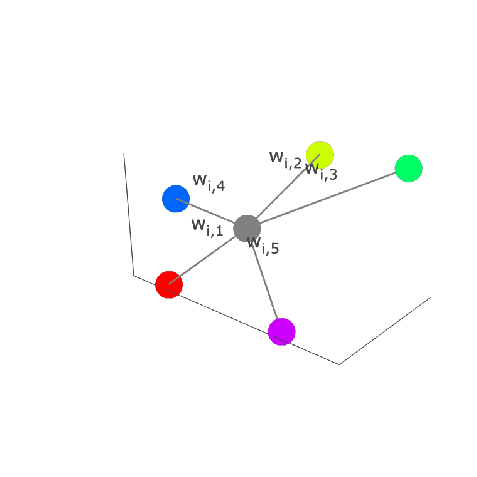
\includegraphics[trim = 40 50 20 20, clip, % left bottom right top
   width = \textwidth]{figures/reconstruction-3d}
 \end{subfigure}
 \hfill
 \begin{subfigure}[b]{0.48\textwidth}
   \centering
   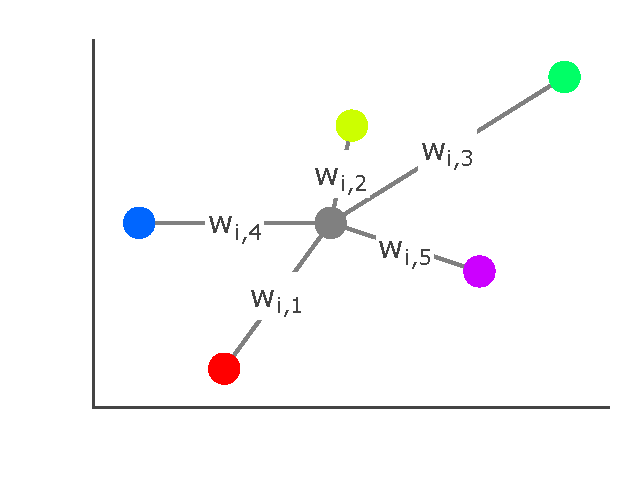
\includegraphics[trim = 20 30 0 20, clip, % left bottom right top
   width = 0.8\textwidth]{figures/reconstruction-2d}
 \end{subfigure}
  \caption[Linear reconstruction in LLE]{Reconstruction in three (\textit{left}) 
  and two (\textit{right}) 
  dimensions, employing the same reconstruction weights. \textit{Source:} own
  representation.}
  \label{fig-reconstruction}
\end{figure}

Algorithmically, LLE performs two subsequent steps \citep{roweissaul2000}:

\begin{tight_enumerate}
  \item Compute the reconstruction weights in $\RD$ minimizing reconstruction 
  loss.
  \item Compute the embedding coordinates in $\Rd$ minimizing embedding loss.
\end{tight_enumerate}

\textbf{Reconstruction loss minimization.}
Reconstruction errors are measured by a quadratic loss function.
Optimization of the objective is subject to a sum-one constraint for the weights
of each point.
A second constraint, zero weights for non-neighboring points, is implicitly
enforced during construction of the neighborhood graph, where edges are only
drawn to vertices belonging to $\x_i$'s neighborhood \citep{ghojoghetal2020}.
The resulting optimization problem is convex and has a unique
closed-form solution\footnote{
Note that the weight matrix $\W$ is different from the one computed in
LEM, but the same symbol is used as not to overload notation.
} \citep{roweissaul2000}:

\begin{equation}
  \begin{split}
    \min_{\W} \varepsilon(\W) &= \min_{\W} \sum_i
    \twonorm{\x_i - \sum_j w_{ij} \x_j} \\
    &= \min_{\W} \sum_i \twonorm{\x_i - \bm{N}_i \bm{w}_i}, \\
    & \text{s.t. } \bm{1}^T \bm{w}_i = 1 \quad \forall i \in \setN.
  \end{split}
  \label{eq-obj-lle-recon}
\end{equation}

Here, $\bm{N}_i \in \R^{D \times k}$ denotes the matrix of feature vectors of
$\x_i$'s neighbors and $\bm{w}_i = \sum_j w_{ij} \in \R^k$.

Equation \ref{eq-obj-lle-recon} can be re-arranged by use of the sum-one
constraint and simplified by introduction of the gram, or local covariance,
matrix $\G_i$ \citep{saulroweis2001}:

\begin{equation}
  \begin{split}
    \min_{\W} \varepsilon(\W) &= \min_{\W} \sum_i \twonorm{\x_i \bm{1}^T
    \bm{w}_i - \bm{N}_i \bm{w}_i} \\
    &= \min_{\W} \sum_i \bm{w}_i^T (\x_i \bm{1}^T - \bm{N}_i)^T
    (\x_i \bm{1}^T - \bm{N}_i) \bm{w}_i \\
    &= \min_{\W} \sum_i \bm{w}_i^T \G_i \bm{w}_i, \\
    & \text{s.t. } \bm{1}^T \bm{w}_i = 1 \quad \forall i \in \setN.
  \end{split}
  \label{eq-obj-lle-recon-2}
\end{equation}

By standard use of a Lagrange multiplier, the solution for the above constrained optimization problem collapses to

\begin{equation}
  \bm{w}_i = \frac{\G_i^{-1}\bm{1}}{\bm{1}^T \G_i^{-1}\bm{1}}.
  \label{eq-obj-lle-sol}
\end{equation}

Solving the reconstruction problem therefore requires $N$ matrix inversions, 
which may prove problematic if the gram matrices do not achieve full rank.
In the case of $D < k$, $\G_i$ is indeed singular and must be robustified by 
adding a small numerical constant to its diagonal \citep{ghojoghetal2020}.
Chapter \ref{challenges} will discuss how this regularization is applied.
\\

\textbf{Embedding loss minimization.}
The second optimization problem minimizes the embedding cost arising from 
mapping neighborhood geometries, derived in the form of reconstruction 
weights, into the $d$-dimensional subspace.
Keeping the weight coefficients fixed, the aim is to find such embedding 
coordinates that best preserve the vicinity structures and adhere to the 
constraints of summing to zero (i.e., being centered around the origin) and 
having unit covariance \citep{roweissaul2000}:

\begin{equation}
  \begin{split}
    \min_{\Y} \Phi(\Y) &= \min_{\Y} \sum_i \twonorm{\y_i - \sum_j w_{ij} \y_j}, 
    \\
    & \text{s.t. } \frac{1}{N} \sum_i \y_i \y_i^T = \I \quad \text{and}
    \quad \sum_i \y_i = \bm{0} \quad \forall i \in \setN.
    % & \phantom{\text{s.t. }} \sum_i \y_i = \bm{0} \quad \forall i \in \setN. 
  \end{split}
  \label{eq-obj-lle-emb}
\end{equation}

The objective can be equivalently stated as an eigenvalue problem.
For this purpose, define $\E = (\I - \W)^T(\I - \W)$ and set 
$\tilde{\Y} = \Y^T$ \citep{cayton2005}, such that:

\begin{equation}
  \min_{\tilde{\Y}} \text{\textit{trace}}(\tilde{\Y}^T \E \tilde{\Y}), \quad
  \text{s.t. } \frac{1}{N} \tilde{\Y}^T \tilde{\Y} = \I \quad \text{and}
  \quad \tilde{\Y}^T\bm{1} = \bm{0}.
  \label{eq-obj-lle-emb-2}
\end{equation}

Again, the solution is found by eigenanalysis of the matrix encoding the 
intrinsic manifold structures.
Note that the first constraint carries a factor $1/N$ as originally 
proposed.
In fact, any such quadratic form, provided its right hand side is of full rank, 
would suffice to ensure the embedding vectors actually span a $d$-dimensional 
space \citep{burges2010}.
The additional sum-zero condition is implicitly met by discarding the constant 
eigenvector associated with the bottom, zero eigenvalue and taking the 
subsequent $d$ eigenvectors to embed the data in $\Rd$ \citep{ghojoghetal2020}.

As mentioned before, the close resemblance to the optimization problem in LEM 
(equation \ref{eq-obj-lem}) is not coincidental.
Recall that LEM builds upon eigenfunctions of the Laplace-Beltrami operator 
$\mathcal{L}$.
\citet{belkinniyogi2003} show that LLE approximates the eigenfunctions of the 
iterated form $\frac{1}{2} \mathcal{L}^2$, which are identical to those of 
$\mathcal{L}$.
Therefore, with a somewhat different intuition, LLE essentially arrives at the 
same conclusion.

% ------------------------------------------------------------------------------

\subsubsection{Hessian Locally Linear Embedding (HLLE)}
\label{hlle}

Lastly, HLLE \citep{donohogrimes2003} pursues an approach toward LGML that 
straddles the two former techniques: it borrows heavily from the idea behind 
LEM but is akin to LLE in an algorithmic sense \citep{dissross2008}.
Proposed under the title \textit{Hessian eigenmaps}, it is therefore also 
referred to as Hessian LLE \citep{donohogrimes2003}.

As opposed to LLE, HLLE is built upon a rigid theoretical foundation.
It makes the assumptions of local isometry and homeomorphicity to an open, 
connected subset of $\RD$ (see chapter \ref{motivation}), which is a much less 
restrictive demand than Isomap's global isometry and parameter space 
convexity \citep{donohogrimes2003}.
With this, HLLE provides veritable convergence guarantees for a wide range of 
cases, albeit only for the continuum limit and not in finite-sample situations 
\citep{cayton2005}.
\\

\textbf{Idea.}
HLLE considers the twice-differentiable mapping functions 
$f: \mani \rightarrow \R$ employed in LEM.
Recall that LEM defines the gradient of $f$ with respect to local tangent 
spaces $T_{\pv}(\mani)$ at $\pv \in \mani$ as a notion of smoothness.
Similarly, HLLE computes the Hessian to measure curviness of $f$ 
\citep{donohogrimes2003}.
One advantage of this modification is that, while the Laplacian equals zero 
for any harmonic\footnote{
An example is indeed given by the coordinate functions; however, other functions 
that are clearly non-linear have the harmonic property (see, for example,
\citet{axleretal2001}).
} function on $\mani$, the Hessian vanishes if and only if $f$ is 
linear \citep{dissross2008}.
\\

\textbf{Hessian functional.}
Consider $\pv \in \mani$ and its $k$-neighborhood $\mathcal{N}_k(\pv)$, each of 
whose members has a unique closest point on $T_{\pv}(\mani)$ via the smooth 
mapping $f$.
Identifying $f(\pv)$ with $\bm{0} \in \Rd$ yields a system of local 
coordinates on $T_{\pv}(\mani)$ that depends on this particular choice of the 
origin.
For the neighbors of $\pv$, let these local coordinates be denoted by 
$\x^{(\text{loc, }\pv)} = \x_1^{(\text{loc, }\pv)}, ..., 
\x_k^{(\text{loc, }\pv)}$.
Then, the Hessian of $f$ at $\pv$ in tangent coordinates may be expressed as the 
ordinary Hessian of a function $g: U \rightarrow \R$, $U$ being a neighborhood 
of zero in $\Rd$ \citep{donohogrimes2003}:

% \begin{equation}
%   (\H_f^{\text{loc})}(\pv))_{i,j} = \frac{\partial}{\x_i}\frac{\partial}{\x_j} 
%   g(\x)\restriction_{\x = 0}
%   \label{eq-hessian-local}
% \end{equation}

% ------------------------------------------------------------------------------

\subsection{Semi-Supervised Locally Linear Embedding (SSLLE)}
\label{sslle}

% ------------------------------------------------------------------------------

\subsubsection{Employment of Prior Information}
\label{prior-info}

% Read belkinniyogi2004 paper on this

\begin{itemize}
  \item Why use labels in the first place?
  \item How will that help?
  \item Exact vs inexact knowledge
\end{itemize}

% ------------------------------------------------------------------------------

\subsubsection{Finding Prior Points}
\label{prior-points}

Prior points: take minmax approach from sparse MDS (Sparse multidimensional 
scaling using landmark points Vin de Silva and Joshua B. Tenenbaum 2004). 
Easy and deterministic after choosing seed value.
Instead Euclidean distances, though, take geodesics as estimated in isomap.

can we view the prior info as some kind of active learning? like we choose 
some points to label in a hopefully cleverish way and then hand them to you 
(e.g., to look at some pictures instead of all droelf thousand)

% ------------------------------------------------------------------------------

\subsubsection{SSLLE Algorithm}
\label{algo-sslle}

\begin{itemize}
  \item What is different wrt standard LLE?
\end{itemize}

% ------------------------------------------------------------------------------

\subsection{Particular Challenges}
\label{challenges}

A number of computational and design-related challenges arise from this 
procedure that must be faced in implementation.
\\

\textbf{Choice of intrinsic dimensionality.} 
Until now, it has been assumed, rather implicitly, that the intrinsic dimension 
$d$ of the data is a known parameter.
This is obviously not always the case in practical applications.
Some methods offer the advantage of estimating $d$ in a built-in fashion. 
PCA, MDS and Isomap, for instance, typically show an indicative gap in their 
eigenvalue spectrum, distinctly pointing out the dimensions with the largest 
share of variability \citep{sauletal2006}.
For LLE, LEM and HLLE, no such tell-tale gap exists.
While \citet{shasaul2005} have indeed drawn a mathematical relation between the 
respective eigenspectra in LLE and LEM and intrinsic data dimensionality, they 
immediately discarded this finding for practical applications due to large 
computational overhead and lack of reliability in finite-sample situations.
There have been various other proposals to tackle the problem of dimensionality 
estimation (for an extensive discussion, see for example 
\citet{disswissel2017}).
However, as the focus of this report lies on a semi-supervised method of 
manifold learning, it is mainly concerned with situations where prior knowledge 
of coordinates, and of $d$ in particular, is actually available.
\\

\textbf{Choice of neighborhood size.} Choosing the size of neighborhoods for 
graph approximation does pose a challenge.
It is a standard hyperparameter optimization problem in which a trade-off 
between locality and overall approximation must be balanced.
If neighborhoods are too small, the model will not be able to learn the global 
manifold structure; with overly large neighborhoods, it will forgo the 
advantages of locality and non-linearity and essentially behave like PCA 
\citep{deridderduin2002}.

\textcolor{red}{Describe applied approach}
\\

\textbf{Robustness of eigendecomposition.} Mainly problem in LLE (?)
\\

\textbf{Computational cost.} Text
\\

\begin{itemize}
  \item Number of neighbors (diss grilli (referenced in lle manual) discusses 
  regression model, ghojogh propose different things)
  \item Intrinsic dimensionality
  \item Singularity of gram matrix (LLE-specific?!)
  \item Large data (landmarks)
\end{itemize}

\textcolor{red}{Comment on difficulty of finding neighbors in high dimensions}
\\
\textcolor{red}{What about using RF proximities for neighbor search? 
Unsupervised RF works with simulating new data from the estimated dist of the 
present ones, see e.g. https://horvath.genetics.ucla.edu/html/RFclustering/RFclustering/RandomForestHorvath.pdf, https://arxiv.org/pdf/2004.02121.pdf}

% ------------------------------------------------------------------------------

\subsection{Comparative Remarks}
\label{comparison}

HLLE has convergence guarantees - not so LLE, LEM (sudderth)
